% ============================================================================
% TP3 -- Reporte de mediciones de RE (entregable OR3)
% Plantilla basada en el TP1 (RE-TP-001). Un solo archivo .tex. Necesita en la
% misma carpeta: logo_fiuba.png, logo_materia.png, las fotos (fig_foto_*.jpg)
% y los datos de los graficos (fig_*.dat), sacados de las trazas del receptor
% del CETEM y de las capturas de la tinySA del EXP-26.
% Compilar con pdfLaTeX (Overleaf: Menu > Compiler > pdfLaTeX).
% ============================================================================
\documentclass[11pt,a4paper]{article}

\usepackage[utf8]{inputenc}
\usepackage[T1]{fontenc}
\usepackage[default]{sourcesanspro}
\usepackage[spanish,es-tabla,es-nodecimaldot]{babel}
\usepackage[a4paper,margin=2.5cm,headheight=14pt]{geometry}
\usepackage{graphicx}
\usepackage{float}       % permite la opcion [H] en figuras y tablas
\usepackage{booktabs}
\usepackage{array}
\usepackage{enumitem}
\usepackage{amsmath}
\usepackage{xcolor}
\usepackage{fancyhdr}
\usepackage{pgfplots}
\pgfplotsset{compat=1.16}
\usepackage[hidelinks]{hyperref}

% ---------------------------------------------------------------- datos ----
\newcommand{\codigo}{OR3}
\newcommand{\version}{1.0 (borrador)}
\newcommand{\fecha}{26 de octubre de 2026}

% Texto que falta completar
\newcommand{\pendiente}[1]{\textcolor{red}{[#1]}}

% Columna de tabla con texto alineado a la izquierda
\newcolumntype{L}[1]{>{\raggedright\arraybackslash}p{#1}}

% Colores de los graficos: series de la paleta de referencia, texto, grilla y referencia neutros
\definecolor{serieuno}{HTML}{2A78D6}
\definecolor{seriedos}{HTML}{EB6834}
\definecolor{serietres}{HTML}{1BAF7A}
\definecolor{tinta}{HTML}{52514E}
\definecolor{gris}{HTML}{A3A29C}
\definecolor{grilla}{HTML}{E4E3DF}
\pgfplotsset{
  espectro/.style={
    width=0.96\textwidth, height=5.2cm,
    grid=major, grid style={grilla,line width=0.4pt},
    axis line style={tinta}, tick style={tinta},
    tick label style={font=\footnotesize,text=tinta},
    label style={font=\small},
    legend style={draw=none,font=\footnotesize,fill=white,fill opacity=0.85,text opacity=1},
    legend cell align=left,
    every axis plot/.append style={line width=0.8pt},
    /pgf/number format/use comma,
  },
}
\tikzset{rotulo/.style={font=\footnotesize,text=tinta,align=center}}

\pagestyle{fancy}
\fancyhf{}
\lhead{\small \codigo{} -- Reporte de mediciones de RE}
\rhead{\small Versión \version}
\cfoot{\small \thepage}

\setlist{itemsep=1pt,topsep=3pt}
\setlength{\emergencystretch}{3em}

\begin{document}

% ============================================================== caratula ====
\begin{titlepage}
  \centering
  \vspace*{0.5cm}
  % logo de la facultad a la izquierda y logo de la materia a la derecha
  \begin{minipage}[c]{0.56\textwidth}
    \centering
    
\includegraphics[width=\textwidth]{logo_fiuba.png}
  \end{minipage}\hfill
  \begin{minipage}[c]{0.34\textwidth}
    \centering
    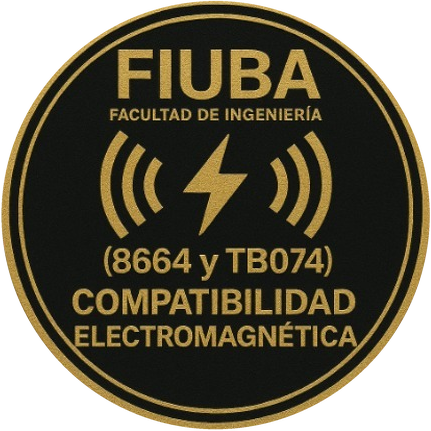
\includegraphics[width=\textwidth]{logo_materia.png}
  \end{minipage}\par
  \vspace{0.8cm}
  {\large Universidad de Buenos Aires -- Facultad de Ingeniería\par}
  {\large Compatibilidad Electromagnética (8664 y TB074)\par}
  {\large Trabajo Práctico N.\textsuperscript{o}~3 -- Entregable OR3\par}
  \vspace{1.6cm}
  {\LARGE \bfseries Reporte de mediciones de RE\par}
  \vspace{0.6cm}
  {\Large Comb Generator basado en Software Defined Radio (SDR)\par}
  \vspace{0.8cm}
  {\large Código: \textbf{\codigo} \qquad Versión: \textbf{\version}\par}
  \vfill
  \begin{tabular}{ll}
    \toprule
    Autor               & Martín Ledesma \\
    Docentes            & Pablo Marino Belcaguy \\
                        & Walter Gustavo Fano \\
    Fecha               & \fecha \\
    \bottomrule
  \end{tabular}
  \vspace{1cm}
\end{titlepage}

% ====================================================== control de cambios ==
\section*{Control de versiones}
\begin{tabular}{@{}llp{8cm}@{}}
  \toprule
  Versión & Fecha & Cambios \\
  \midrule
  0.1 (borrador) & 21 de octubre de 2026 & Plantilla. \\
  1.0 (borrador) & \fecha & Mediciones en casa (12-10) y en el CETEM (13-10). La comparación con CISPR~11 queda sin terminar. \\
  \bottomrule
\end{tabular}

\section*{Participantes}
\begin{tabular}{@{}lp{10cm}@{}}
  \toprule
  Persona & Función \\
  \midrule
  Martín Ledesma        & Autor. Operó la SDR en las dos ocasiones. \\
  Federico Martinez     & Operó la cámara, el mástil y el receptor del CETEM. \\
  Pablo Marino Belcaguy & Docente, revisión. \\
  Walter Gustavo Fano   & Docente, revisión. \\
  \bottomrule
\end{tabular}

\tableofcontents

% ============================================================================
\section{Introducción}

Este reporte presenta las mediciones de emisiones radiadas hechas con el generador peine basado en la SDR bladeRF 2.0 micro xA9, en dos ocasiones. La primera fue en casa, el 12 de octubre de 2026, para comprobar que el peine se irradia y se recibe con margen. La segunda fue en la cámara semianecoica del CETEM, el 13 de octubre, donde además se midió el Comb generator de la tesis de otro alumno como referencia. En las dos el peine salía a 0~dBm por cable, el nivel del EXP-25, así que estas mediciones sirven para conocer la fuente y la repetibilidad del montaje, pero no para compararlas con un límite. El procedimiento de ensayo está en el RE-TP-001 (TP1) y la placa se describe en el manual de la SDR (TP2).

% ============================================================================
\section{Montaje}

\begin{table}[H]
  \centering
  \small
  \begin{tabular}{@{}L{3.0cm}L{4.9cm}L{6.1cm}@{}}
    \toprule
    & Casa (12-10-2026) & CETEM (13-10-2026) \\
    \midrule
    Lugar & Interior de una casa, sin blindaje & Cámara semianecoica, SDR sobre la mesa \\
    Distancia & 2~m & 3~m \\
    Peine & 24 líneas de 60 a 980~MHz, una cada 40~MHz, a 0~dBm por cable (EXP-25 y EXP-26) & El mismo \\
    Antena de la SDR & Telescópica de 30~cm, extendida & Telescópica de 30~cm, extendida y vertical \\
    Recepción & tinySA Ultra con su antena de 10~cm, de 45 a 1005~MHz & Receptor R\&S ESR-7 con antena bilog en mástil, a 1, 2 y 3~m de altura \\
    Configuración & Atenuación automática & De 30~MHz a 1~GHz, RBW de 120~kHz, detector de pico, MAX HOLD y preamplificador de 20~dB \\
    \bottomrule
  \end{tabular}
  \caption{Montajes.}
\end{table}

\begin{figure}[H]
  \centering
  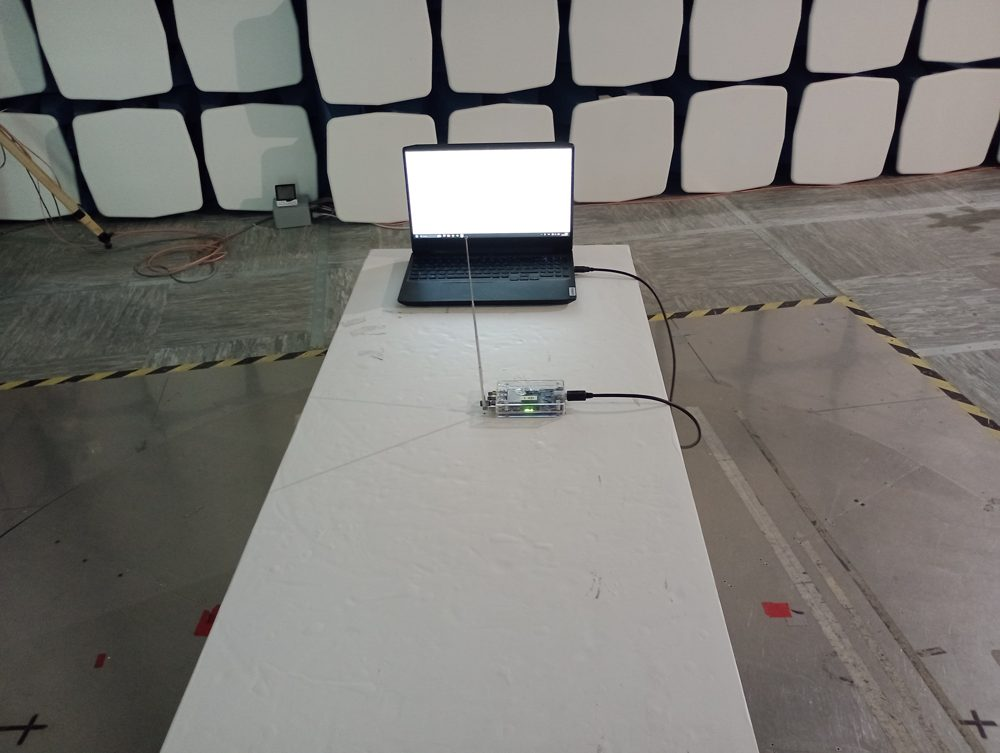
\includegraphics[width=0.32\textwidth]{fig_foto_sdr.jpg}\hfill
  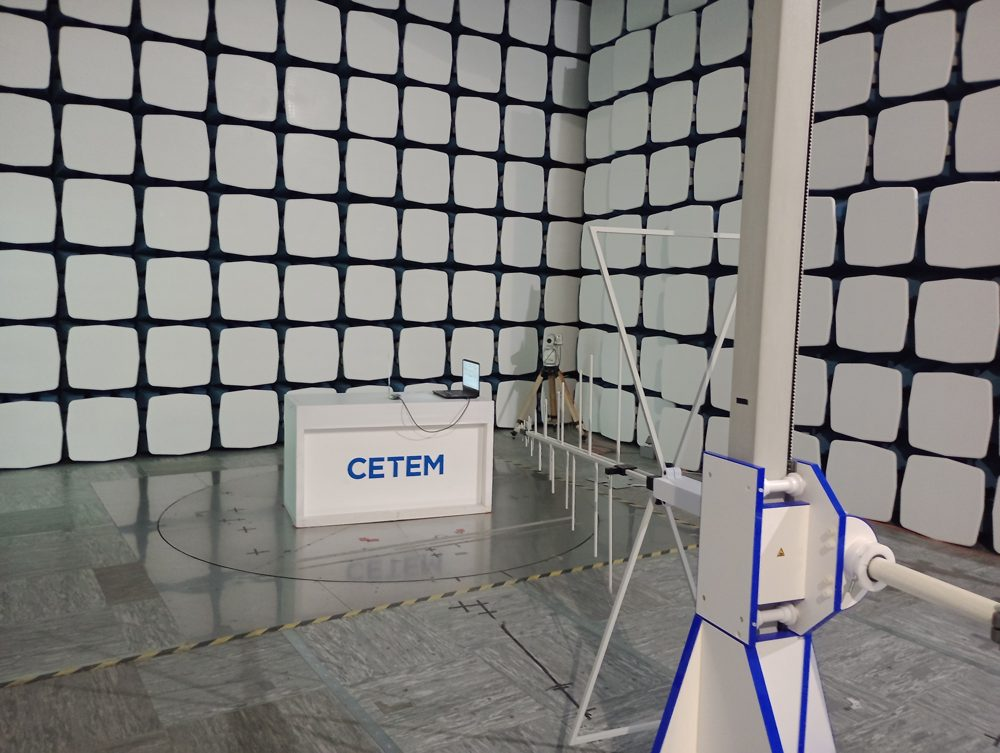
\includegraphics[width=0.32\textwidth]{fig_foto_antena.jpg}\hfill
  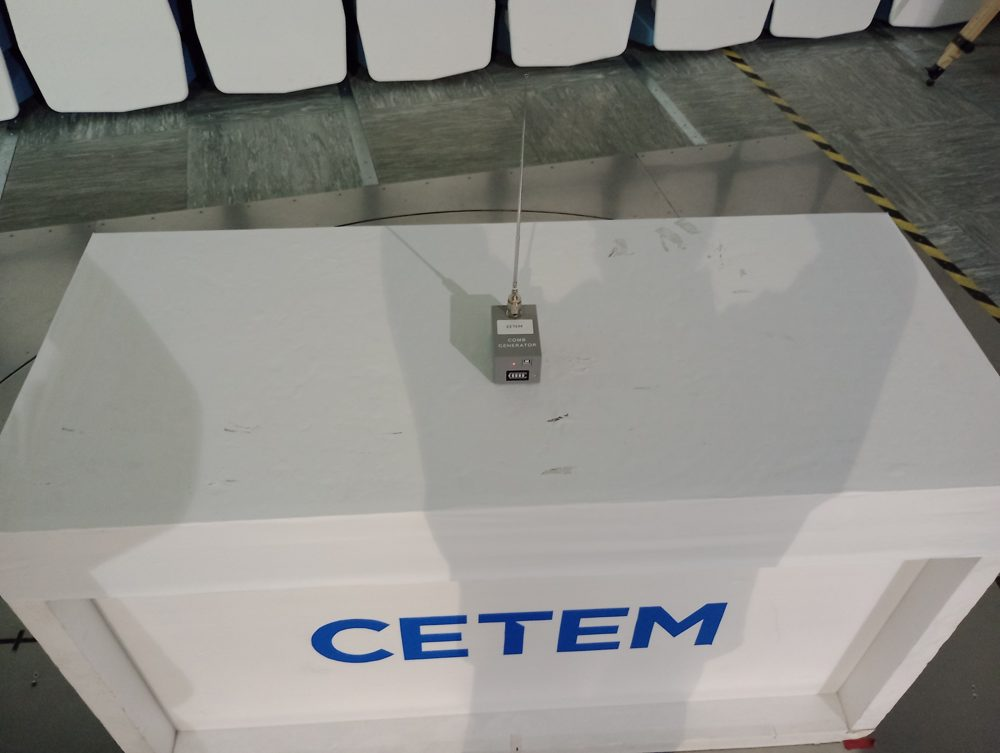
\includegraphics[width=0.32\textwidth]{fig_foto_comb.jpg}
  \caption{Montaje en el CETEM. A la izquierda, la SDR con su antena y la notebook sobre la mesa. En el centro, la antena de medición en el mástil frente a la mesa. A la derecha, el Comb generator.}
\end{figure}

En el CETEM la SDR emitiendo y sin antena se midió con 20~dB de atenuación en el receptor, y el Comb generator, la SDR en pausa y el piso de la cámara con 10~dB. Con 20~dB el piso sube unos 10~dB. Para que las trazas sean comparables, a las medidas con 10~dB se les sumaron 10~dB, de modo que todos los pisos quedan en el mismo lugar. Sin ese ajuste, las diferencias contra esas trazas serían 10~dB mayores. Las alturas de la antena de medición y la posición de la mesa se tomaron de los nombres de los archivos del receptor. La notebook quedó dentro de la cámara, sobre la misma mesa que la SDR y con un USB corto, aunque el procedimiento la preveía afuera.

% ============================================================================
\section{Mediciones en el CETEM}

\subsection{La SDR y su emisión propia}

\begin{figure}[H]
  \centering
  \begin{tikzpicture}
    \begin{axis}[espectro, xmin=30, xmax=1000, ymin=10, ymax=105,
        xlabel={Frecuencia (MHz)}, ylabel={Campo (dB$\mu$V/m)},
        legend pos=north east, legend columns=3]
      \addplot[gris] table[x=f,y=pausa]{fig_sdr_1m.dat};
      \addplot[seriedos] table[x=f,y=sinantena]{fig_sdr_1m.dat};
      \addplot[serieuno] table[x=f,y=antena]{fig_sdr_1m.dat};
      \legend{{En pausa}, {Sin antena}, {Con antena}}
    \end{axis}
  \end{tikzpicture}
  \caption{SDR en vertical con la antena de medición a 1~m de altura, emitiendo con antena, emitiendo sin antena y en pausa.}
  \label{fig:sdr}
\end{figure}

\begin{itemize}
  \item Las 24 líneas se vieron a las tres alturas, entre 69 y 96~dB$\mu$V/m.
  \item A 1~m de altura quedan de 30 a 56~dB sobre la SDR en pausa (figura~\ref{fig:sdr}).
  \item Sin antena la placa igual irradia, con las líneas entre 31 y 57~dB$\mu$V/m.
  \item La respuesta de la cadena, del nivel radiado contra el conducido, varía unos 20~dB a lo largo de la banda.
\end{itemize}

\subsection{Comparación con el Comb generator}

\begin{figure}[H]
  \centering
  \begin{tikzpicture}
    \begin{axis}[espectro, xmin=30, xmax=1000, ymin=10, ymax=105,
        xlabel={Frecuencia (MHz)}, ylabel={Campo (dB$\mu$V/m)},
        legend pos=north east, legend columns=2]
      \addplot[seriedos] table[x=f,y=comb]{fig_comb.dat};
      \addplot[serieuno] table[x=f,y=sdr]{fig_comb.dat};
      \legend{{Comb generator}, {SDR}}
    \end{axis}
  \end{tikzpicture}
  \caption{SDR y Comb generator en vertical, con la antena de medición a 1~m y la mesa en 0°.}
  \label{fig:comb}
\end{figure}

El Comb generator, con su látigo vertical y una línea cada 10~MHz, se vio con 90 de sus 95 líneas de 50 a 990~MHz a 6~dB o más sobre el piso, entre 41,5 y 67~dB$\mu$V/m (figura~\ref{fig:comb}). En las mismas frecuencias la SDR emite una mediana de 33~dB más. Girar la mesa casi no cambia el nivel del Comb generator, con una mediana de 1~dB, y en horizontal prácticamente no se ve.

\subsection{Repetibilidad}

\begin{figure}[H]
  \centering
  \begin{tikzpicture}
    \begin{axis}[espectro, xmin=40, xmax=1000, ymin=60, ymax=100,
        xlabel={Frecuencia de la línea (MHz)}, ylabel={Campo (dB$\mu$V/m)},
        legend pos=south west, legend columns=3]
      \addplot[serieuno, mark=*, mark size=1.3pt] table[x=linea,y=h1]{fig_alturas.dat};
      \addplot[seriedos, mark=*, mark size=1.3pt] table[x=linea,y=h2]{fig_alturas.dat};
      \addplot[serietres, mark=*, mark size=1.3pt] table[x=linea,y=h3]{fig_alturas.dat};
      \legend{{Antena a 1~m}, {A 2~m}, {A 3~m}}
    \end{axis}
  \end{tikzpicture}
  \caption{Nivel de cada línea de la SDR con la antena de medición a tres alturas, en vertical y con la mesa en 0°.}
  \label{fig:alturas}
\end{figure}

\begin{itemize}
  \item Al cambiar la altura de la antena, cada línea varía una mediana de 7,8~dB y hasta 15,8~dB, por el reflejo en el piso de la cámara (figura~\ref{fig:alturas}).
  \item Con la mesa girada 180° y la antena a 3~m, las líneas bajan una mediana de 2,9~dB, entre $-8{,}8$ y +1,8~dB.
  \item Con la antena a 1 y 2~m, varias portadoras (línea + 10~MHz) aparecen a menos de 6~dB de su línea, 9 a 1~m y 6 a 2~m, y algunas incluso la superan. A 3~m quedan de 31 a 43~dB abajo, como por cable.
  \item Hay picos sueltos casi al nivel de las líneas, en 265, 885 y 944~MHz y otras frecuencias, que no aparecen con la SDR en pausa. Su causa no está confirmada, y falta saber si el silencio entre saltos estaba activado.
\end{itemize}

% ============================================================================
\section{Medición en casa}

\begin{figure}[H]
  \centering
  \begin{tikzpicture}
    \begin{axis}[espectro, xmin=45, xmax=1005, ymin=-100, ymax=-35,
        xlabel={Frecuencia (MHz)}, ylabel={Nivel (dBm)},
        legend pos=north east, legend columns=2]
      \addplot[gris] table[x=f,y=ambiente]{fig_casa.dat};
      \addplot[serieuno] table[x=f,y=peine]{fig_casa.dat};
      \legend{{Ambiente}, {Peine calibrado}}
    \end{axis}
  \end{tikzpicture}
  \caption{Peine recibido a 2~m con la tinySA y su antena de 10~cm, y el ambiente con la SDR desconectada (EXP-26).}
  \label{fig:casa}
\end{figure}

En casa el piso quedó en $-91$~dBm y las líneas se recibieron entre $-52$ y $-75$~dBm de 220 a 980~MHz (figura~\ref{fig:casa}). De las 24 líneas, 20 superaron al ruido por 10~dB o más y 18 por 20~dB o más, hasta 38~dB en 660~MHz. A esa distancia no sirven las de 60 y 140~MHz, que no se ven, la de 100~MHz, tapada por la FM, y la de 180~MHz, con solo 6~dB.

El ambiente tiene FM cerca de 100~MHz y telefonía celular entre 718 y 772~MHz. Con el peine aparece además un pico en 751~MHz, 3~dB bajo la línea de 740~MHz y en la frecuencia de su portadora, que ya se había visto por cable en el EXP-24. Un primer intento quedó inválido porque la tinySA tenía 30~dB de atenuación fija y solo 6 líneas superaban el piso. No se midió el peine sin calibrar ni se repitió el montaje, así que la repetibilidad en casa queda pendiente.

% ============================================================================
\section{Comparación con CISPR 11}

\pendiente{Sección sin terminar. Faltan las mediciones de diciembre de 2026.}

Las mediciones de este reporte se hicieron con el peine a 0~dBm por cable, muy por encima del nivel para el que está pensada la comparación, así que contrastarlas con el límite no aporta. La comparación con CISPR~11 grupo~1 clase~A se hará con las mediciones de la visita al CETEM de diciembre de 2026, con el peine calibrado del EXP-28 y el procedimiento RE-TP-001.

% ============================================================================
\section{Conclusiones}

\pendiente{Sección sin terminar. Faltan las mediciones de diciembre de 2026.}

% ============================================================================
\section{Referencias}

\begin{enumerate}
  \item RE-TP-001, Procedimiento de ensayo de emisiones radiadas (TP1 de este proyecto).
  \item OE2, Manual y procedimiento funcional de la SDR (TP2 de este proyecto).
  \item CISPR~11:2024, límites de emisiones para equipos industriales, científicos y médicos.
  \item Rohde \& Schwarz, receptor de EMI R\&S ESR, manual de uso.
  \item tinySA Ultra, manual de uso.
\end{enumerate}

\end{document}
